\documentclass[main.tex]{subfiles}
% BACKGROUND
%
%\newglossaryentry{poly}{name={Polynomial},description={An Algebraic Function of the form $\sum_{i=0}^{N} a_i x^i$ where $N$ is the degree of the polynomial, $a_i \in \Re$ is the i^{th} coefficient and $x$ is the independent variable.}}

% rename to Background and Project
\begin{document}
    
  It is important, in order to understand the significance of this project, to know that it is only the first phase in a larger project. The larger project should, in short, be able to identify different physical phenomena that occur in Oil and Gas wells, based on the data available from these wells. Correct and timely identification has the potential to pre-empt structural damage that would impede production, as well as shed light on yet illusive processes that, at this time, very little data is available for.
  \\\\
  \Cref{fig:well} shows a temperature-depth curve from an Oil well. This is the type of data that should be analysed. However, of each well there are several of these curves taken per day and the larger project should ultimately be able to analyse the two dimensional data sets that are created from these. 
  
  \begin{figure}[h]
    \centering
    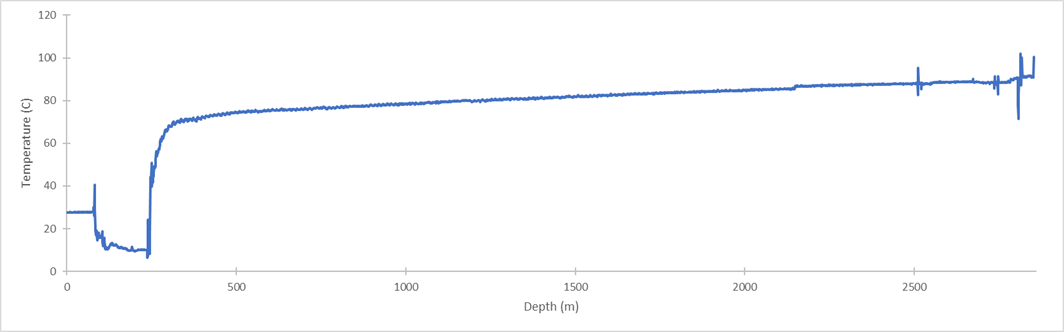
\includegraphics[width=\linewidth]{figures/wellData}
    \caption{Temperature data from an Oil-Well in the North-Sea. Temperature is taken in approximately one meter intervals along the piping of the well, beginning on the oil rig, with 2860 data points shown. \\
    A number of phenomena can be identified on the graph, but most visibly the entry point of the well into the sea floor at about 200m (where the temperature grows sharply), a bias at about 2200m and a number of outliers to the right of 2500m. These phenomena should be characterised as discussed in \cref{sec:POI}. Separate regression analysis after cleaning away noise finds that the data is likely to be logarithmic at approx. 285-370m (R=0.97) and linear thereafter (R=0.96).
    \\\\
    Data by Curtecy of HyperDap.}
    \label{fig:well}
  \end{figure}
  
  \section{Requirement Specification}
  
    Based on examples of the available data and the appearance of these phenomena in the data, it was pointed out by a number of future project participants, that in most of these phenomena the derivative of the data may largely provide all the necessary information to at least pinpoint these phenomena and mark them for further analysis. Given the simplicity of numerical derivatives it was decided that this would be explored first.
    \\\\ 
    This project is to provide an assessment of the viability of a derivative based analysis of the available data, and create a prototype software that can serve as the foundation for further analysis. As such the following functional Requirements were agreed:
    
    \begin{enumerate}
      \item \label{it:requ:classify} (Must) Create software that can classify data sets into mathematical types.
      \item \label{it:requ:recAnalysis} (Must) Provide recommendations to expand and build on this analysis.
      \item \label{it:requ:recQual} (Should) Provide recommendations to improve the quality of classification.
      \item \label{it:requ:data} (Should) Create a prototype framework for the data to be represented internally, independently from the customer's data representation.
      \item  \label{it:requ:interp} (Could) Begin to build on data classification to extract further information from the data.
    \end{enumerate}
    
    While Requirement \ref{it:requ:recQual} mostly refers to the software's ability to deal with noise, it also hints at possible processing and memory improvements.
    \\\\
    Particularly Requirement \ref{it:requ:interp} remained intentionally vague, as at the time the nature of this further analysis was unknown (hence Requ. \ref{it:requ:recAnalysis}).
    
    Non-functional requirements were sightly more specific, to the extend to which the larger project was already defined.
    
    \begin{enumerate}
      \item \label{it:requ:java} The software must be in Java11 if possible, and usable from a Java 11 environment if that is not possible.
      \item \label{it:requ:calculus} The method of analysis should make use of calculus and focus on low level computation. Metaphorically it should provide the building blocks or the foundation for further analysis.
      \item \label{it:requ:license} The software must be free of licence fees or other costs due to intellectual property.
      \item \label{it:requ:deppend} Dependencies should be kept to a minimum whenever possible.
      \item \label{it:requ:softDevel} Best software engineering practice should be followed to allow the software to be further developed without spending time on preventable quality improvement.        
    \end{enumerate}
    
    Requirements \ref{it:requ:java}, \ref{it:requ:license} and \ref{it:requ:deppend} in combination meant that, for the most part, very few  libraries could be taken advantage of. Much of the mathematics, in particular that will be recommended for further analysis, can be outsourced to various libraries, but most of these are not available for Java, and those that are have been lagging behind in updating to 11. 
    \\\\
    While Requirement \ref{it:requ:softDevel} may appear rather redundant, given the exploratory nature of the project it simply means that not all considerations should be focused on experimentation, but good quality software is ultimately the goal, which makes use of the methods that I am experimenting with.
    
  \section{Project Management}
  
    While throughout the project a form of AGILE project management was upheld as much as possible, the project plan and even objectives have been subject to a number of changes (see \Cref{tbl:timeline}). This did require a degree of flexibility in project management, however, as thus far it has been a one person project this flexibility is practically guaranteed.
    
    \begin{table}[h]
      \centering
      \caption{The timeline of the honours project, broken down into phases of up to one month. Note how before the project commenced it was intended to refactor and improve an existing physical simulation/emulation with a somewhat detailed project plan in existence. This simulator has been a component of the \textit{intelligent Hydrate Platform}, owned by \textit{BlueGentoo}. The Project Objective evolved from here due to various circumstances.}
      \begin{tabularx}{\linewidth}{ X | X c }
        \hline
        \thead{Time Period} & \thead{Objective} & \thead{Activity} \\
        \hline \hline
        \makecell*{Before \\ Late-January} & \makecell*{Refactor iHP \\ Simulator} & Planning and Research. \\ \hline
        
        \makecell*{Up to \\ Mid-February} & \makecell*{New Synthetic \\ Data Generator} & Planning and Inception \\ \hline
        
        \makecell*{Late-February and \\ Early March} & \makecell*{Calculus Data \\ Analysis} & Planning, Inception and Research \\ \hline
        
        \makecell*{March} & \makecell*{Calculus Data \\ Classification} & Data Format R\&D \\ \hline
        
        \makecell*{Late-March to \\ Early-April} & \makecell*{Calculus Data \\ Classification} & Classification R\&D \\ \hline
        
        \makecell*{Early-April} & \makecell*{Calculus Data \\ Classification} & Finalisation of Software \\ \hline   
        
        \makecell*{Remaining April} & \makecell*{Calculus Data \\ Classification} & Validation, Documentation and Presentation \\ \hline
        
        \hline
      \end{tabularx}
      \label{tbl:timeline}
    \end{table} 
    
    \subsection{Shifting Objectives}
  
      Initially the Objective was to refactor and improve an existing simulation that was part of another O\&G  project, the \textit{intelligent Hydrate Platform} (iHP). Within this project it was important to emulate the behaviour of natural gas production for development and testing. The project was expected to begin development of Machine Learning components and an improved simulation would have benefited this development. However, due to lack of engagement by the customer and subsequent stalls in development, this project objective became rather infeasible, as it would have relied extensively on information from the client that was not available.
      \\\\
      Initially my intention was to continue to build on my experience and research regarding synthetic data generation for the iHP, and create a flexible simulation module. This new synthetic data generator would be able to generate different data sets based on user definitions of analytical representations, with realistic and adjustable noise. The intention was to prepare a flexible simulation module that could be applied not to one but to many domains. This would have been rather ambitious, but more importantly would likely exceed the time available for this honours project. While significant progress would have been made, it is unlikely that further development would have been possible, and this unfinished project would not have been of use to anybody.
      \\\\
      Finally, an opportunity opened up in the above mentioned \textit{HyperDap} project to help analyse large data sets of O\&G production data. This project essentially applies the inverse of the previously planned one, extracting an analytical representation from sets of real data. It  offered a number of prospects compared to the two previous plans. \textit{HyperDap} was much more forthcoming in providing information, with example data sets provided almost immediately, and my supervisor at university continuously updated me with more information provided by the client. It also offered an opportunity for the resulting software to be applied in a real world context alongside a job offer to continue development beyond the scope of this honours project.
    
    \subsection{Development}
    
      Once the project's objective was finally well defined initial focus was on the design and implementation of a data representation, followed by the more challenging design of the classification method outlined in \Cref{cha:conc}. In each of these phases development naturally followed a waterfall-esk AGILE model. The development of the Data Format in particular passed through a number of different variations before arriving at the basic idea discussed in \Cref{sec:impl:dataPrinciple} from which the currently implemented family of classes was developed.
      \\\\
      The classification method described in \Cref{cha:conc} on the other hand was rather straight forward to implement once inception was completed. During inception, however, it was necessary to ensure the method would be conceptually sound, which would then be partially confirmed in subsequent tests.
      \\\\
      In order to properly demonstrate the software one week in mid-April was dedicated to the development of a data generator and GUI, which would allow a user to observe the results of analyses by the software. While these modules were intended for demonstration purposes, they proved useful in much more rigorous testing and debugging of the classifier, as it visualised its output very well.
      \\\\
      Finally the project was subject to two types of documentation. As a component of good practice software was documented in javadoc as it was developed, with the exception of GUI components and parts of the generator, as these were intended solely for demonstration originally. In April, however, the project was documented for university marking, producing this report and a presentation. Within the latter documentation the project was reviewed and some additional tests performed.
      
      \subsubsection*{Technology Use}
        
        For the duration of this project the same technologies were used that will likely be mandatory for the future HyperDap project.
        
        \paragraph{Version Control and Backup} was provided by \textit{GitHub} and \textit{GitDesktop} v1.6.5. The repository can be found at \href{https://github.com/SonkeWohler/analyser}{https://github.com/SonkeWohler/analyser}.
        
        \paragraph{The Integrated Development Environment} used was \textit{Eclipse} v4.9.0, making use of the appropriate extensions to allow proper development in Java11 and any other components, while making use of the \textit{Open JDK} v11.0.2.
        
        \paragraph{Dependency Management} was conducted using \textit{Apache Maven} v3.6, which also provided \textbf{packaging and deployment} functionality.
        
        \paragraph{Unit Testing} was performed with \textit{JUnit}, while conceptual testing was carried out  manually.
        
        \paragraph{Team Management} was not an issue for this one person project, but collaboration with my supervisor, as well as development notes not kept in the above environments, made use of \textit{Trello} and \textit{Google Drive}, as well as, to some extend, \textit{Microsoft Excel}.
        
        
    
\end{document}
